\documentclass[12pt,a4paper]{article}

\usepackage{setspace}
\onehalfspacing
\usepackage{caption}
\usepackage{subcaption}
\usepackage{float}
\captionsetup[table]{font={stretch=1.5}}     %% change 1.5 as you like
\captionsetup[figure]{font=onehalfspacing}    %% change onehalfspacing as you like
\usepackage[english]{babel}
\usepackage[utf8]{inputenc}
\usepackage{amsmath}
\usepackage{mathtools}
\usepackage{amssymb}
\usepackage{graphicx}
\usepackage{braket}
\usepackage[colorinlistoftodos]{todonotes}
\usepackage[top=1.0in,left=1.0in,right=1.0in,bottom=1.0in]{geometry}
\usepackage[
backend=biber,
style=numeric,
citestyle=ieee,
subentry,
mcite=true,
]{biblatex} %biblatex, more modern form of bibtex 
\usepackage{multicol,caption}
\usepackage{makeidx}
\usepackage{pdfpages}
\usepackage[compat=1.0.0]{tikz-feynman}
\usepackage{hyperref}
%\usepackage{LuaLaTeX}
\makeindex
%\usepackage{fixltx2e}
%\usepackage{cite} %if you want to use bibtex
\newenvironment{Figure}
  {\par\medskip\noindent\minipage{\linewidth}}
  {\endminipage\par\medskip}
\setlength{\columnsep}{1cm}
\setlength{\parindent}{0pt}
\usepackage{color,soul}
\usepackage{booktabs}
\newcommand{\ra}[1]{\renewcommand{\arraystretch}{#1}}
\defbibentryset{griffiths2008book}{griffiths2008introduction, griffiths2008neutrino1.5, griffiths2008neutrinoOscillations} %if you want to use biblatex with multiple referances, useful for books
\addbibresource{refs.bib} %if you want to use bib latex, add sources
\setlength\bibitemsep{2.0\itemsep} % if you want to use bib latex and increase item seperation

\title{Rough Thesis}
\date{\today}
\author{Ronald Collins ID:200948843}

\begin{document}
\maketitle

\begin{Figure}
 \centering
 
\includegraphics[width=1.0\linewidth]{Liverpool_logo}
 \captionof*{figure}{} 
\end{Figure}


\begin{center}
\textit{Department of Physics, High Energy Physics\\}
\textit{VIDARR collaboration\\}
\end{center}


\pagenumbering{gobble}
\newpage
\pagenumbering{roman}
\begin{abstract}
\normalsize A basic overview\\

\providecommand{\keywords}[1]{\textbf{\textit{Keywords:}} #1} %Keywords command has to be supplied manually
\keywords{Monte Carlo, Geant4, High performance computing (HPC), Anti-neutrino}
\end{abstract}
\vspace{5mm} %5mm vertical space before main body of text
%\begin{multicols}{2}
\tableofcontents
\newpage

\pagenumbering{arabic}

\section{The Aim Of VIDARR} \label{sec_theAimOfVidarr}
The aim of the VIDARR project is to demonstrate the potential usefulness of a plastic scintillating detector for safeguarding purposes. To that end the characterisation and simulation of two versions of the detector will be used in order to show the full potential of this idea. Reactor monitoring using $\Bar{\nu_e}$ was suggested as early as 1978 \cite{Borovoi_1978} but the political climate of the cold war era prevent interest in the technology from being fully realised. In the modern political climate where nuclear power is seen as a stable form of low carbon power generation more nations are considering the technology once again. And as such the concern of the proliferation of atomic weapons has increased. Current methods of non-proliferation are dependent on accurate bookkeeping and empirical measurement estimations from power generation. Whilst these methods are effective more direct methods of measuring the flux from reactors and thereby the production of weapons grade material would greatly aid in the trust between nations and help to prevent the spread of atomic weaponry. 
\\\\This technology also has benefits for increasing the burn-up of nuclear waste which could increase power generation at nuclear power plants and reduce the production of nuclear waste which has to be stored. This potential is not yet fully realised due to the increased complexity of the method as it requires differentiating between different isotopes rather than just measuring flux. Tough this should be feasible it is not possible to test this capability until the upgraded VIDARR detector is deployed at a reactor site. 

\section{The Prototype Detector}\label{sec_thePrototypeDetector}
This thesis will cover two distinct versions of the detector. The original prototype detector which was re-purposed technology from the T2K ND280 ECal \cite{Allan_2013} and an upgraded version which uses the same basic materials in the detector but upgraded electronics and containment which will be refereed to as the ``Verification Instrument for Direct Assay of Nuclear Reactors at Range'' (VIDARR) detector. The rest of this section will focus on the prototype detector.
\\\\As it is the basis for the other detectors a quick overview of the T2K ND280 ECal will be required. The ND280 is series of detectors from the neutrino oscillation experiment T2K which relies on a $\mu_nu$ beam entering the detector as show in figure \ref{fig_nd280Fig}. This detector was comprised of several different types of detector including time projection chambers (TPCs) and fine-grained detectors (FGDs) and electromagnetic calorimeters (ECals) \cite{Allan_2013}. The ECals are of particular interest as they are the basis for the prototype and VIDARR detectors. 
\begin{figure}[H]
 \centering
 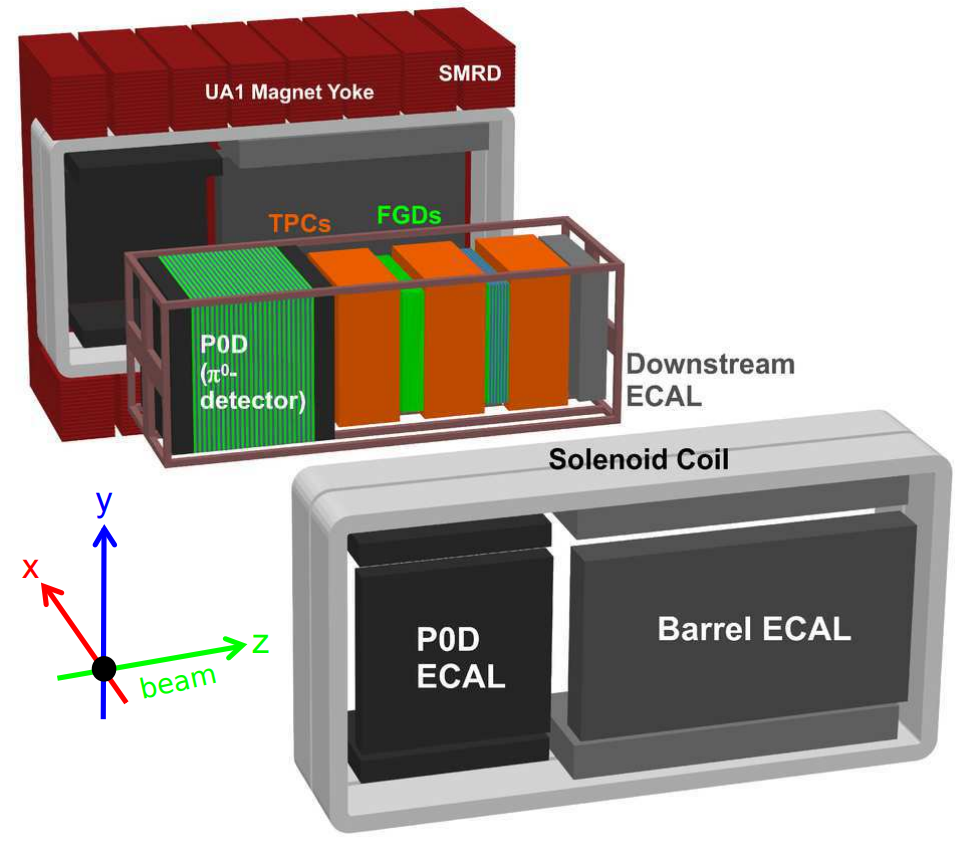
\includegraphics[width=\linewidth/2]{ND280Fig.png} 
 \captionof{figure}{Diagram of the ND280 detector. From \cite{Allan_2013}} %~can be used as a kind of place holder in latex
 \label{fig_nd280Fig}
\end{figure}
The T2K Ecals were made from plastic scintillating bars measuring 4\,cm by 1\,cm with varying lengths arranged in alternating layers at 90 degrees to each other \cite{Allan_2013}. Wavelength shifting (wls) fibres were placed in the centre of the scintillating bars which shift the wavelength from blue to green \cite{Allan_2013}. These wavelength shifting fibres are then connected to multi-pixel photon counters (MPPCs) which are the instrument which reads out the signal. This signal is then read in by Trip-T front-end electronic boards (TFBs) which then splits the signal into different cycles each containing 1.5 microseconds of information. All of this is shared by the prototype detector. 
\\\\However a crucial different between the ECals of the ND280 and the prototype detector is that the (ECals) had a layer of lead in between each of the plastic scintillating layers \cite{Allan_2013}. In the prototype this has been replaced with a layer of gadolinium so that neutrons were capture for inverse $\beta$ decay. The prototype was also designed to fit inside of a shipping container each bar having a length of 152\,cm and the whole detector measuring 152\,cm by 152\,cm with 49 layers of plastic scintillating bars totalling 49\,cm. The electronic systems were also adapted from the from the T2K system however they were altered such that they triggered on a gadolinium cascade from inverse $\beta$ decay. There were 23 cycles numbered from 0-22 with 0-17 cycles being considered "prompt" and cycle 18 is the trigger cycle. Cycles 19 -22 were left alone so that they could be compared in case time dependent issues arose from the altered system. Cycles 19-22 are useful for $\mu$ tomography as time dependent errors can arise from this adaptation of the electronics. 
\\\\The original detector was deployed at Wylfa power station in Anglesey Wales for an 18-month period. This run proved successful measuring the power on from the reactor to within good agreement to the measured reactor flux see figure \ref{fig_prototypeMeasumentFlux}. With a measured anti-neutrino rate of 172.1 $\pm$ 4.6 candidates per day when the reactor is off and 203.7 $\pm$ 19.6 when the reactor was on \cite{Carroll_2018}. Unfortunately due to cooling issues with the prototype the reactor shutdown was not observed. This is one of the main motivating factors behind the upgrade of the detector as the first generation MPPCs and reporposed electronics were susceptible to high levels of noise if the temperature was not carefully controlled. 
\begin{figure}[H]
 \centering
 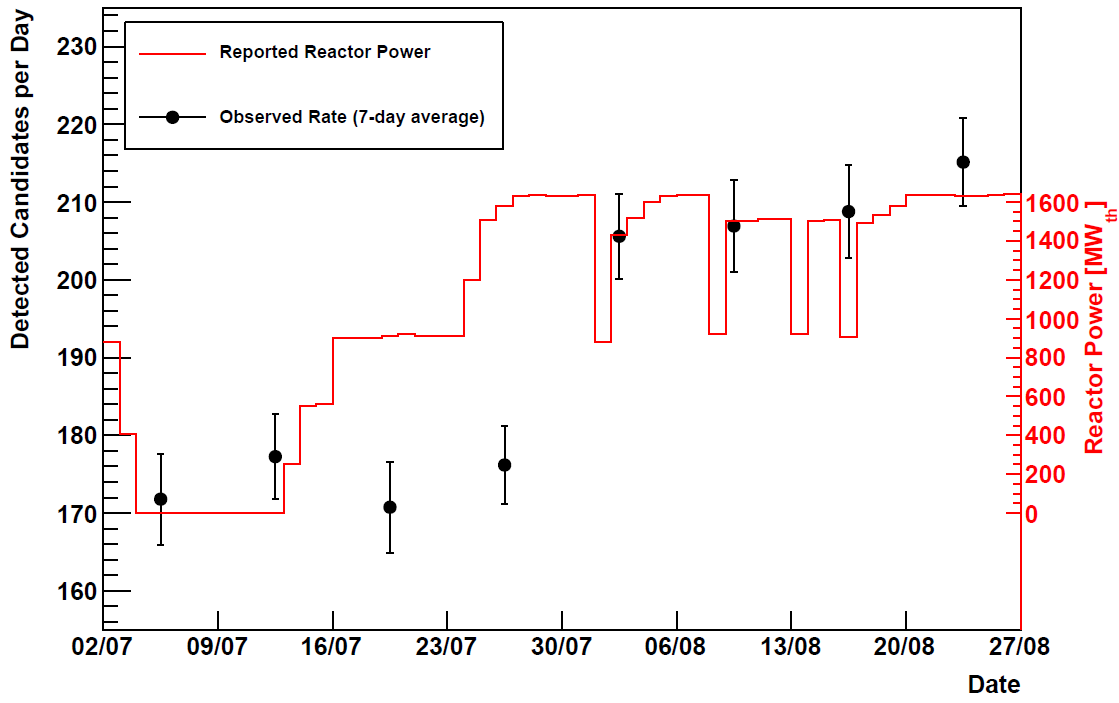
\includegraphics[width=0.90\linewidth]{prototypeMeasureOnFig.png} 
 \captionof{figure}{Measured anti-neutrino flux compared to the power generation from the Wylfa power station. From \cite{Carroll_2018}} %~can be used as a kind of place holder in latex
 \label{fig_prototypeMeasumentFlux}
\end{figure}
\section{The Upgraded Detector}\label{sec_theUpgradedDetector}
Please note that in the following section of text the term upgraded and VIDARR detector are used interchangeably. The upgraded detector will have 21 more layers than the previous detector going from 49 to 70 layers and the 3 missing columns in side a are also now instrumented. This means the number of channels have increased from 1793 to 2660 which results in an increase of mass by $\sim$ 50\,\%, thus improving the fiducial volume of the detector. This means that more energy from the gadolinium cascade is contained within the detector thus allowing for more effective noise reduction when triggering. Therefore the increase in layers will allow for a higher efficiency of neutron capture. The increase in layers will not yield a significant increase in positron efficiency as positrons are effectively contained to a $\sim$ 99\,\% level with both 1793 channels and 2660 channels as they are contained within 1-2 bars.
\\\\The electronics have also been improved significantly compared to the original detector. The original electronics were carried over from the T2K Ecal, they were the first generation of the technology with relatively high noise rates compared to the current generation used in the VIDARR detector. The energy resolution of the electronics have been greatly increased \hl{(any quantifiable numbers for this stuff?)}. And the noise rates for the original electronics were also more susceptible to changes in temperature than the electronics in the upgraded detector. In addition the upgraded detector will also have field-programmable gate array (FPGA) boards which connect with analogue boards which in turn connect to the MPPCs. The use of FPGA boards allow for more complex trigger functions to be used with up to two thresholds to be used and allows for the summed energy and the number of bars to be hit to be used for trigger discrimination. Which should allow for better signal to noise discrimination than the original detector.
\\\\A basic cut investigation used a form of machine learning called a support vector machine (SVM) to determine the best cut and which dimensions gave the best separation. The cut was dominated by the number of bars hit at the lower threshold of 0.1\,MeV, the most accurate cut would have been utilising the number of bars hit above 0.1\,MeV and the summed energy above the 0.1\,MeV threshold. However due to the structure of the FPGA boards and their programming it was more prudent to use the number of bars hit above both the 0.1\,MeV thresholds and 0.5\,MeV threshold. The cost in classifier accuracy was minimal and it allowed for faster development of the FPGA firmware. 
\\\\To lessen temperature fluctuations in the VIDARR detector the cooling in and around the detector module has been greatly increased from the prototype. The original detector had six radiator fins on 2 sides of the detector which were primarily aimed at cooling the TFBs on each fin. The upgraded VIDARR detector will also have these fins which will help cool the new boards but on the same 2 sides as the fins there will also be two new radiators behind the fins which run the width and height of a side. Greatly increasing the speed that heat will dissipate inside the detector. This will allow for a more consistent temperature  thus reducing dark noise even further from the MPPCs. 
\section{GEANT 4 Simulation}\label{sec_geant4Simulation} 
\subsection{GEANT4 Overview}\label{subSec_geant4Simulation_g4Overview}
The VIDARR detector is also represented in a GEANT4 simulation which is a provident physics simulation package. According to the GEANT4 collaboration GEANT4 ``covers a comprehensive range including electromagnetic, hadronic and optical processes and a large set of long-lived particles materials and elements over a wide energy range starting in some cases from 250\,eV and extending in others to the TeV range'' \cite{Agostinelli:2002hh}. Considering that the energy range for inverse $\beta$ decay is 2\,MeV-8\,MeV \cite{Mueller_2011} this simulation package appears to meet the needs of the VIDARR collaboration. However whilst the simulation of the resulting positrons is reasonably simplistic the simulation of the neutrons is more challenging due to the difficulty in simulating the Gadolinium cascade. 
\subsection{Gadolinium Cascade}\label{subSec_geant4Simulation_gdCascade}
The Gadolinium cascade is difficult to measure and accurately simulate for for two main reasons. The first is that the gadolinium nuclei that have good neutron capture are isotopes $^{155}$Gd and $^{157}$Gd which have 155 and 157 nucleons respectively. Both of these nuclei are large and as such it is difficult to accurately model the individual interactions between each of the nucleons. So, there is no agreed upon model at present for the absorption and emission of the 8\,MeV $\gamma$ cascade. The second issue is that the high energy $\gamma$ rays emitted by the cascade are very difficult to contain. Therefore, getting accurate measurements and energy efficiencies for the cascade is also very difficult. These two problems compound one another it is difficult to measure the cascade so it is difficult to model which, in turn, makes it difficult to know the energies expected to be emitted by the nuclei. Further issues are caused by highly penetrative making efficiency estimates even less accurate. \hl{(No references... whilst this is all reasonably straight forward some more concrete numbers and figures would be nice...)}. Gadolinium is used because of its high efficiency (10$\%$ - 40$\%$) compared to other neutron capturing materials such as $^6$Li which only has about $1\%$ \cite{Abdushukurov_2010}. 
\\\\The simulation has several distinct modes: cosmic $\mu$, noise, and inverse $\beta$ decay. The cosmic mode has a realistic distribution \hl{what paper did Matt Murdock use to form the realistic distribution?} and a cosmic hemisphere distribution. The cosmic hemisphere distribution is used to check that the analysis chain is functioning as expected and for testing simulated reactor shadows. In all other cases the realistic cosmic distribution is used when simulating cosmic $mu$s. The noise distributions are random uniform distributions from 0 - 10\,MeV simulating which cover $p$,$\bar{p}$,$\pi^+$,$\pi^-$,$e^-$,$e^+$, $\alpha$,$\bar{\alpha}$,$n$. The IBD simulation is done by simulating a positron between 0 - 10\,MeV and then simulating at $\sim$ 10 $\mu$s later a neutron. \hl{Timing plot required!}. The range 0 - 10\,MeV is used instead of 2 - 8\,MeV to allow the testing of edge cases and for better fitting and or particle identification later down the road. \hl{need figures for both cosmic and ibd, this requires access to OLL however...}.
\subsection{Modelling Attenuation}\label{subSec_geant4Simulation_ModellingAttenuation}
In order to characterise the physical effects of the detector at test stand was set up by fellow collaborator George Holt. This test stand contained a single plastic scintillating bar where a caesium 137 source was placed at 11 intervals across the bar from which attenuation of the 662\,KeV peak could then be measured. This is then shown in figure \ref{fig_attenuationPlot} this exponential decay is then put into the simulation so that the amount of light produced is more physical. 
\begin{figure}[H]
 \centering
 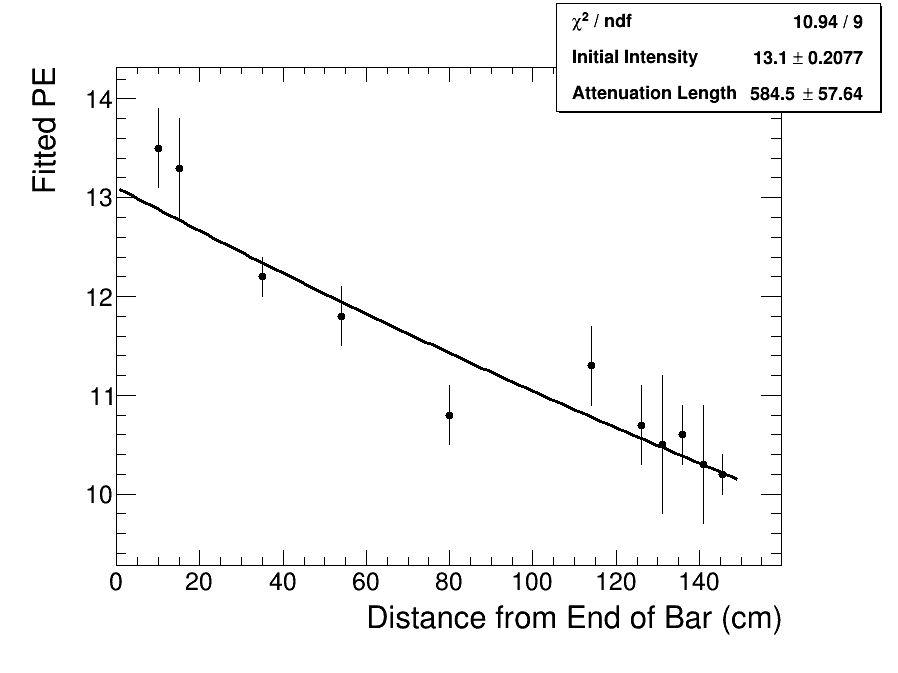
\includegraphics[width=1.0\linewidth]{result_from_attnPlotter.png} 
 \captionof{figure}{The attenuation plot for test stand produced by George Holt. The attenuation length is 580 $\pm$ 60 \hl{units!}} %~can be used as a kind of place holder in latex
 \label{fig_attenuationPlot}
\end{figure}

\subsection{Modelling Dark Noise}\label{subSec_geant4Simulation_ModellingDarkNoise}
Another data driven physical effect modelled in the simulation is the dark noise. Depending on the temperature of the room the electronics in an MPPC will give signals that are non-physical. The dark noise was measured at room temperature by George Holt over a 12 hour period the results in figure \ref{fig_pureDarkNoise} show peaks in units of photo-electrons (PE) with peaks for 1\,PE, 2\,PE and 3\,PE being clearly visible. The MPPC was put inside a container where no light would reach the sensor. 
\begin{figure}[H]
 \centering
 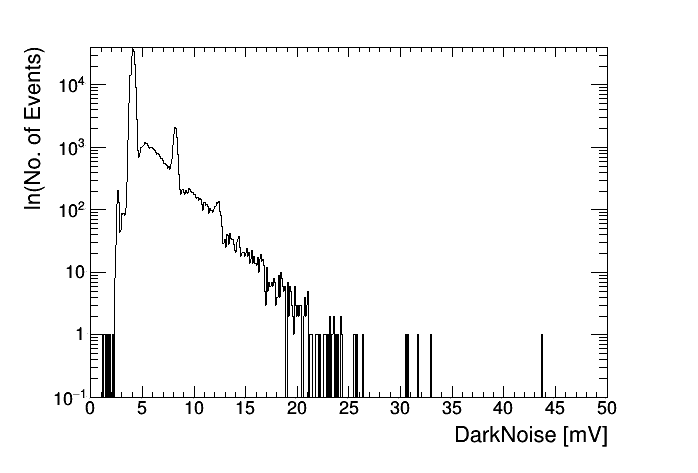
\includegraphics[width=0.8\linewidth]{pureDarkNoise_output.png}
 \captionof{figure}{Dark Noise from the MPPC taken over a period of $\sim$ 12\,hrs. The PE peaks for 1\,PE 2\,PE and 3\,PE can be seen at 4.1\,mv, 8.2\,mv and 12.3\,mv respectively. } %~can be used as a kind of place holder in latex
 \label{fig_pureDarkNoise}
\end{figure}

The dark noise has two distinct components, the peaks and the background surrounding the peaks. The background surrounding the peaks can be modelled using an exponential fit and is done so in figure \ref{subFig_expFitOfDark}. The pedestal peak is also removed and then the exponential is used past 13.7\,mV which can be seen in figure \ref{subFig_fittedDarkNoise}. 
\begin{figure}[H]
\centering
\begin{subfigure}{.5\textwidth}
  \centering
  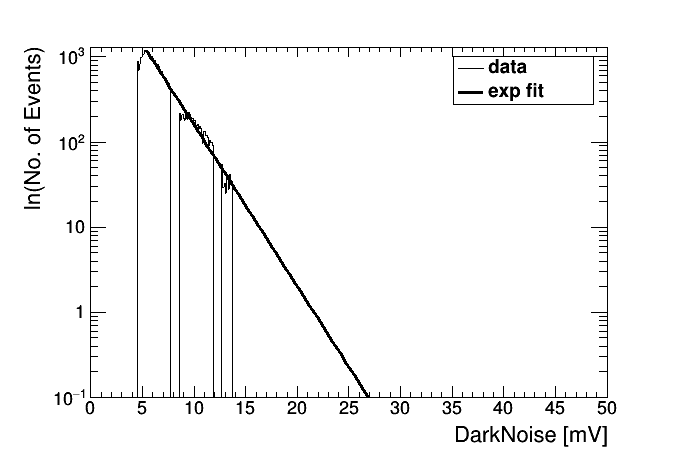
\includegraphics[width=\linewidth]{fit_of_dark_noise.png}
  \captionsetup{width=.9\linewidth}
  \caption{Fit of exponential function using TFit to fit the after-pulsing of the MPPCs}
  \label{subFig_expFitOfDark}
\end{subfigure}%
\begin{subfigure}{.5\textwidth}
  \centering
  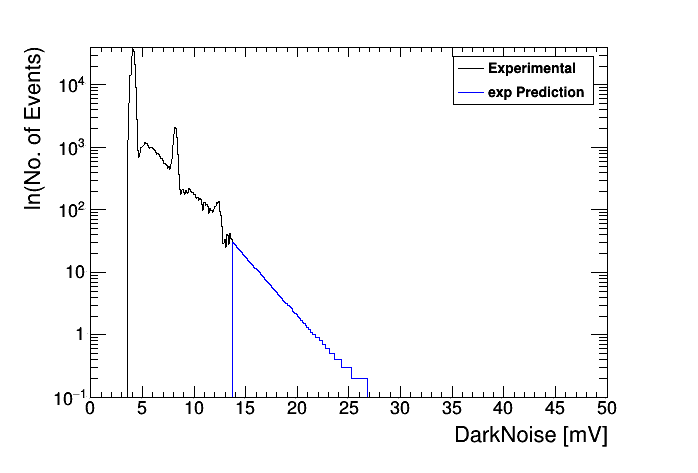
\includegraphics[width=\linewidth]{fittedDarkNoise_output.png}
  \captionsetup{width=.9\linewidth}
  \caption{Fitted exponential past 13.7\,mv once the number of events dropped below 10.}
  \label{subFig_fittedDarkNoise}
\end{subfigure}
\caption{Dark Noise from the MPPC taken over a period of $\sim$ 12\,hrs with an exponential fitted, with a $\chi ^2$ /DOF = 159.748}
\label{fig_fitting_of_non_peak_dark_noise}
\end{figure}

The results from \ref{fig_fitting_of_non_peak_dark_noise} can then be used to construct a cumulative distribution seen in figure \ref{fig_cumulative_prob_dark}, this cumulative distribution is what is used by the simulation in order to reconstruct the dark noise distribution. During the simulation a random dice is thrown that probability is then converted back into a dark noise value which is then assigned to a random bar in the detector. Values past 13.7\,mV use the exponential fit.
\begin{figure}[H]
 \centering
 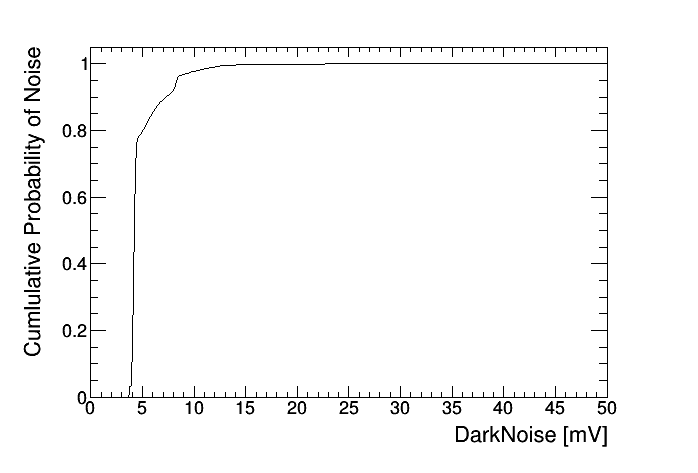
\includegraphics[width=0.8\linewidth]{cumulative_prob_dark_noise.png}
 \captionof{figure}{cumulative probability of the dark noise, which is converted to a table and then searched using the golden section search} %~can be used as a kind of place holder in latex
 \label{fig_cumulative_prob_dark}
\end{figure}
\hl{would be really nice if I could produce a histo of the simulated dark noise and quantify what that looks like and how much we're expecting when we deploy}

\subsection{Modelling Light Emission}\label{subSec_geant4Simulation_ModellingLightEmission}
In order to measure light for a given amount of scintillating material we need to consider several factors. For organic scintillators the type of particle has a significant effect on the absolute light yield. The response of organic scintillators to charged particles can best be described by a relation between $dL/dx$ the fluorescent energy emitted per unit path length and $dE/dx$ the specific energy loss for the charged particle.  A widely used relation first suggested by Birks \cite{birks_1964} is based on the assumption that a high intonation density along the track of the particle leads to quenching from damaged molecules and a lowering of the scintillation efficiency. If we assume that the density of damage molecules along the wake of the particle is directly proportional to the ionisation density we can represent their density by $B(dE/dx)$ where $B$ is a proportionality constant. Birks assumes that some fraction $k$ of theses will lead to quenching\cite{knoll_2010}. A further assumption is that in absence of quenching the light yield is proportional to energy loss shown in equation \ref{equ_light_yield_proportional}. $S$ is the normal scintillation efficiency. To account for the probability of quenching birks then writes equation \ref{equ_Birks_formula}. Equation \ref{equ_Birks_formula} is commonly referred to as Birks formula. As a practical matter the product $kB$ is treated as an adjustable parameter to fit experimental data for a specific scintillator whereas $S$ is particle specific which provides absolute normalisation \cite{knoll_2010}.  
\begin{equation}
\frac{dL}{dx} = S\frac{dE}{dx}
\label{equ_light_yield_proportional}
\end{equation}
\begin{equation}
\frac{dL}{dx} = \frac{S\frac{dE}{dx}}{1 + kB \frac{dE}{dx}}
\label{equ_Birks_formula}
\end{equation}
\\\\In this model molecules in the ionisation column are labelled ``damaged'' and ``undamaged'' for convenience where ``damaged'' molecules are those which dissipate ionisation energy nonradiatively (quenching) and so lower scintillation efficiency\cite{craun_1970} \cite{knoll_2010}. ``Damaged'' molecules occupy highly ionised or excited states, they de-excite quickly ($<$ 1 ns) to the ``undamaged'' condition \cite{craun_1970}. Some permanent damage will occur and does contribute to long term degradation of the scintillator but is not relevant for quenching\cite{craun_1970}. From this B is the ratio of ``damaged''/``undamaged'' molecules and k is the relative probability of quenching. kB is treated as a single adjustable parameter as there is no way to measure k or B separately \cite{craun_1970} \cite{knoll_2010}. Where kB is scintillator dependant only and will be refereed to as a single entity as Birk's constant. The response for electrons above $\sim$ 125\,keV is linear \cite{craun_1970}. This is also seen in Birk's law which also becomes linear for fast electrons \cite{knoll_2010}. This is important for modelling electrons. 
\subsection{MINERvA Birk's Constant}\label{subSec_geant4Simulation_MINERvA_Birks_Constant}
In equation \ref{equ_Birks_formula} the parameters $kB$ and $S$ are empirically determined. $S$ is a normalisation parameter that is particle dependent and kB is the birks constant for the scintillator and is particle independent. The MINERvA collaboration \cite{aliaga_2015} also uses the same scintillator as the VIDARR detector \cite{aliaga_2014}, the collaboration determined the value of the of kB to be 0.0905 $\pm$ 0.015\,mm/MeV at best fit. This Birks parameter was obtained by using GEANT4 MC data, which is the same approach by which VIDARR has obtained its birks parameter.
Both the VIDARR and MINERvA approach use the Geant4 bertini cascade model when attempting to measure the \\\\Birks parameter $kB$ \cite{Heikkinen_2003}. In addition both use the QGSP physics list which applies the quark gluon string model when simulating particles \cite{Patrick_2018}. The steps have to remain course in Geant4 otherwise the $kB$ parameter changes  \cite{aliaga_2015}. This is why the EMY physics lists were not used, even though they simulate smaller steps and so would potentially simulate stopping better. Then energy range for the MINERvA signal is of order $\sim$ 1\,GeV, whereas the energy range for VIDARR's signal is 0-10\,MeV. However a major source of noise for VIDARR are cosmic muons which have energies $\sim$ 1\,GeV and protons with energies between 0-10\,MeV as a result of fast neutrons. Using the minerva data requires going to higher energies (lower $dE/dx$) in order to ensure similar results in the $dL/dx$ fit.  
\\\\The results of the MINERvA Birks law investigation concluded that a birks constant of 0.0905 $\pm$ 0.015\,mm/MeV was the most accurate value for the scintillator \cite{aliaga_2015}. Whilst the MINERvA experiment measures protons with an energy range of 0\,MeV-500\,MeV and the particles of VIDARR's interest are $\overline{\nu_{e}}$s with energy range between 0\,MeV-10\,MeV the Birk's constant is the same regardless. This is because the Birk's law is a representation of the scintillator itself and therefore is not particle or energy dependent, the amount of saturation in the scintillator that the Birks constant represents is constant in all cases. 

\subsection{Loss of Deposited Energy due to Quenching}\label{subSec_geant4Simulation_quenching_loss}
\hl{Very Important!: This work is currently not replicable, the collection of scripts is on my hepstore somewhere and needs to be backed up and put onto git as soon as possible!}
\\\\The effect of quenching varies greatly depending on the particle it is a function of both energy and mass. By considering three example particles and their corresponding anti-particles the scale of quenching can be observed. The first particle to consider would be electrons as they are one of the most common sources of noise and have a large charge to mass ratio when compared to other particles that could be potential background for this experiment. The level of quenching for electrons and positrons is very minimal which can be seen in figure \ref{fig_electron_positron_quenched_and_not}. This was simulated using a ``slab'' of material, figure \ref{fig_electrons_viewed_in_slab}, instead of using a bar or a full detector this was done to ensure that all of the energy was kept inside the plastic scintillator so that the full energy loss due to quenching could be measured. 

\begin{figure}[H]
\centering
\begin{subfigure}{.5\textwidth}
  \centering
  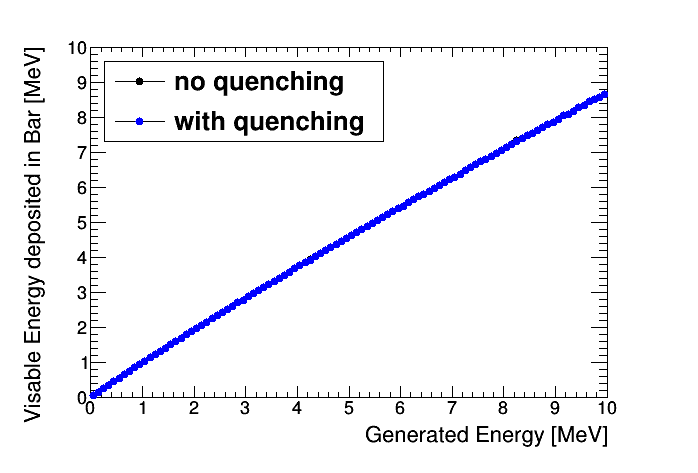
\includegraphics[width=\linewidth]{quench_eng_LinElectrons.png}
  \captionsetup{width=.9\linewidth}
  \caption{Visible electron energy deposition with and without quenching}
  \label{subFig_electron_quenched_and_not}
\end{subfigure}%
\begin{subfigure}{.5\textwidth}
  \centering
  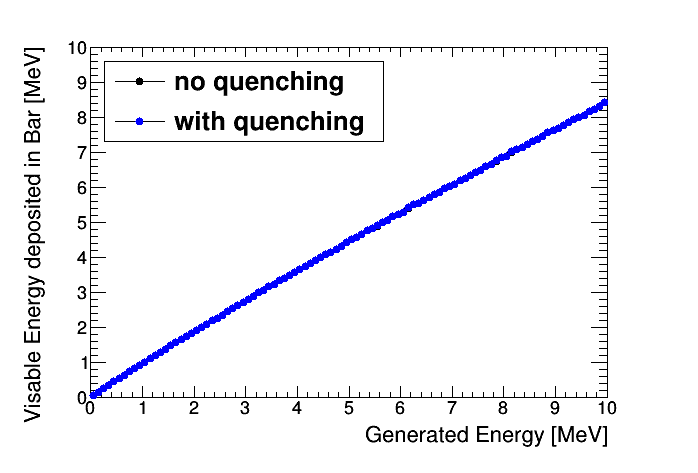
\includegraphics[width=\linewidth]{quench_eng_LinPositrons.png}
  \captionsetup{width=.9\linewidth}
  \caption{Visible positron energy deposition with and without quenching}
  \label{subFig_positron_quenched_and_not}
\end{subfigure}
\caption{Electrons and positrons visible energy with and without quenching in a ``slab'' of material}
\label{fig_electron_positron_quenched_and_not}
\end{figure}

\begin{figure}[H]
\centering
\begin{subfigure}{.5\textwidth}
  \centering
  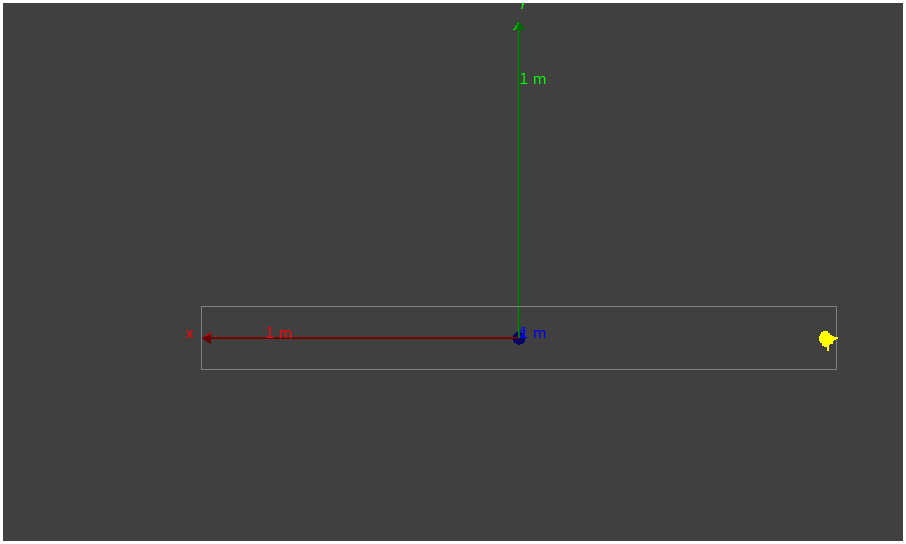
\includegraphics[width=\linewidth]{e-_10MeV_Length_on_view.png}
  \captionsetup{width=.9\linewidth}
  \caption{electrons side on view in ``slab''}
  \label{subFig_electron_side_slab}
\end{subfigure}%
\begin{subfigure}{.5\textwidth}
  \centering
  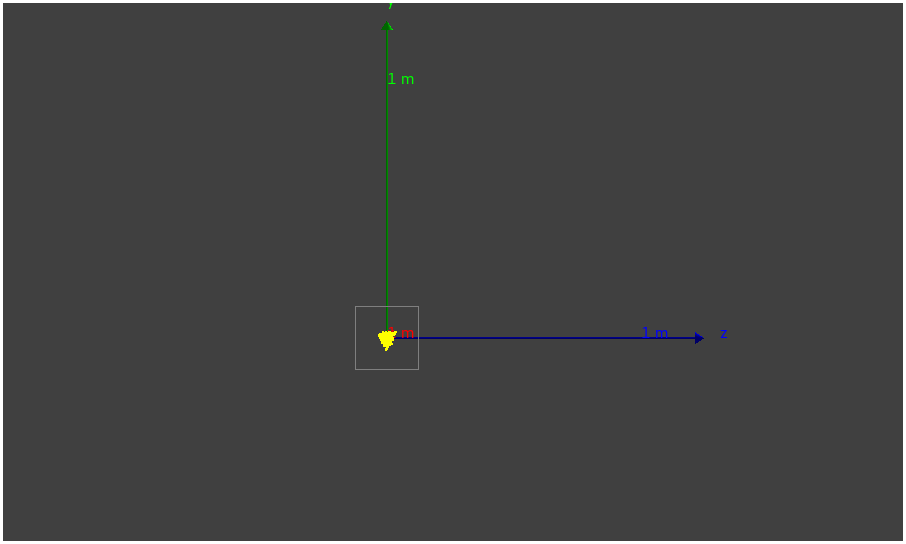
\includegraphics[width=\linewidth]{e-_10MeV_side_on_view.png}
  \captionsetup{width=.9\linewidth}
  \caption{electron length on view in ``slab''}
  \label{subFig_electron_length_slab}
\end{subfigure}
\caption{Electron side and length on view in ``slab'' of material, the electrons are not leaving the material.}
\label{fig_electrons_viewed_in_slab}
\end{figure}

The effect of quenching on protons is much more significant than for electrons, this is because the charge for protons is equal and opposite for electrons but the mass is $\sim$ 2000 times greater than for electrons. This results in a large amount of energy no longer being deposited in the scintillator which can be seen in figure \ref{fig_proton_Apronton_quenched_and_not} which shows both the energy deposition of protons and anti-protons. In figures \ref{subFig_proton_quenched_and_not}, \ref{subFig_Aproton_quenched_and_not} the energy deposition is linear for protons and anti-protons without quenching this suggests that the majority of the energy lost is lost via quenching. For $\alpha$ particles the effect is even more significant $\alpha$ particles which are 4 times more massive than protons but have twice the charge. The effect of quenching is $\sim$ 4 times greater for $\alpha$ particles than for protons which can be seen when comparing the energy deposited in the slab for figures \ref{fig_proton_Apronton_quenched_and_not} and \ref{fig_alpha_Aalpha_quenched_and_not}. 

\begin{figure}[H]
\centering
\begin{subfigure}{.5\textwidth}
  \centering
  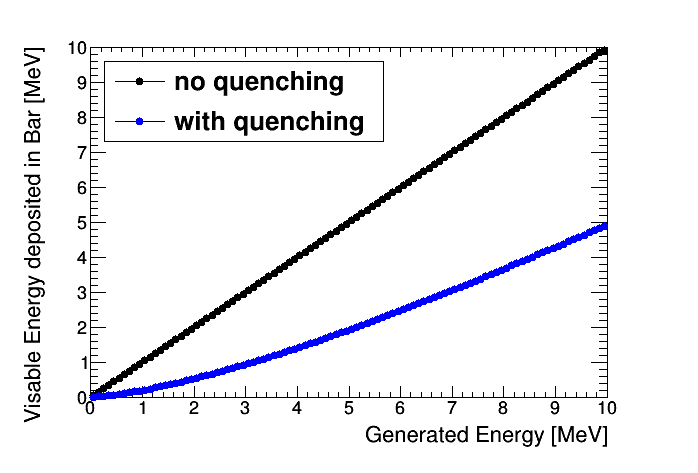
\includegraphics[width=\linewidth]{quench_eng_protons.png}
  \captionsetup{width=.9\linewidth}
  \caption{Visible proton energy deposition with and without quenching}
  \label{subFig_proton_quenched_and_not}
\end{subfigure}%
\begin{subfigure}{.5\textwidth}
  \centering
  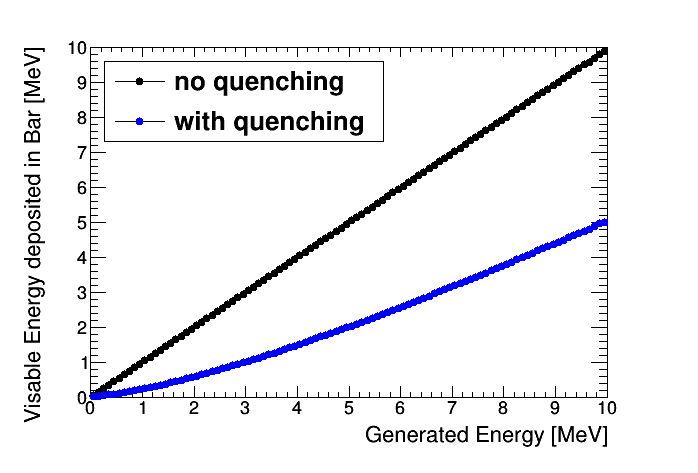
\includegraphics[width=\linewidth]{quench_eng_Aprotons.png}
  \captionsetup{width=.9\linewidth}
  \caption{Visible anti-proton energy deposition with and without quenching}
  \label{subFig_Aproton_quenched_and_not}
\end{subfigure}
\caption{protons and anti-protons visible energy with and without quenching in a ``slab'' of material}
\label{fig_proton_Apronton_quenched_and_not}
\end{figure}

\begin{figure}[H]
\centering
\begin{subfigure}{.5\textwidth}
  \centering
  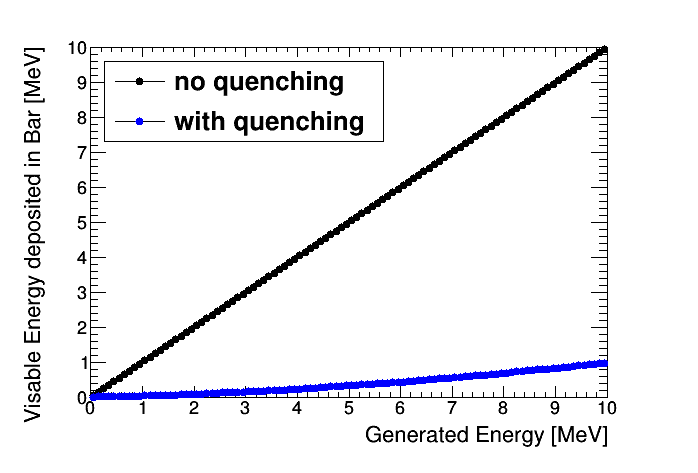
\includegraphics[width=\linewidth]{quench_eng_Alpha.png}
  \captionsetup{width=.9\linewidth}
  \caption{Visible alpha particle energy deposition with and without quenching}
  \label{subFig_alpha_quenched_and_not}
\end{subfigure}%
\begin{subfigure}{.5\textwidth}
  \centering
  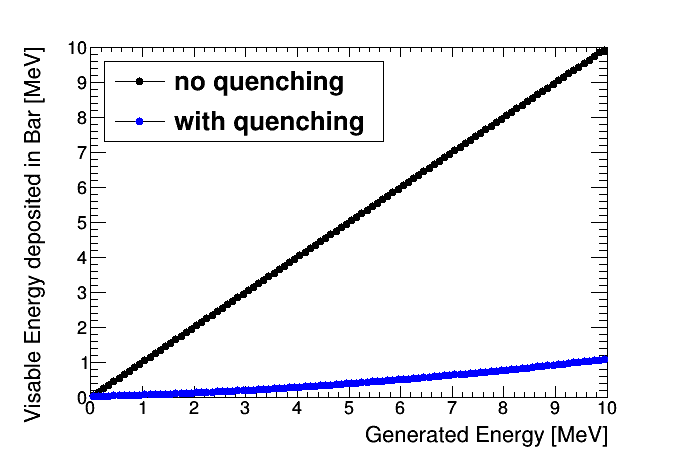
\includegraphics[width=\linewidth]{quench_eng_AAlpha.png}
  \captionsetup{width=.9\linewidth}
  \caption{Visible anti-alpha particle energy deposition with and without quenching}
  \label{subFig_Aalpha_quenched_and_not}
\end{subfigure}
\caption{alpha and anti-alpha particles visible energy with and without quenching in a ``slab'' of material}
\label{fig_alpha_Aalpha_quenched_and_not}
\end{figure}

\subsection{Monte Carlo Modelling of Birks Law}\label{subSec_geant4Simulation_monte_carlo_birks_law}
\hl{Very Important!: This work is currently not replicable, the collection of scripts is on my hepstore somewhere and needs to be backed up and put onto git as soon as possible!}
\\\\The photon model in Geant4 is computationally expensive as the simulation toolkit simulates optical photon tracks at every energy deposition for a given amount of energy. With a scintillation yield of $10^5$\,ph/MeV as in this simulation the slowdown observed at higher energies is extreme. This slowdown can be somewhat alleviated by counting the number of photons and then killing the optical photon tracks, as it is the number of photons produced that determines quenching, but even this is still computationally expensive. So whilst the count and kill method was used for determining Birk's law, once the light was characterised the count and kill method was abandoned due to its high computational load.
\\\\In order to accurately quantify the response of Birks law Monte Carlo modelling was used in Geant4. This was done so that the value of $S$ in equation \ref{equ_Birks_formula} could be found for each particle. The Geant4 physics list of QGSP\_\_BERT\_\_HP allows for good repdouction of Birk's law \cite{Patrick_2018},\cite{aliaga_2015}. However, two new models of the scintillator were required in order to accurately quantify the effects of the Birk's constant, both of them required the removal of all wavelength shifting fibres and MPPCs and so are just scintillator. The first model was a ``slice model'' that was 1\,mm thick and had a cross section of 0.2\,m by 0.2\,m, this allowed for the approximations $dL/dx \approx \Delta L / \Delta x$ and $dE/dx \approx \Delta E / \Delta x$ to be used. The second model was a ``slab'' model (figure \ref{fig_electrons_viewed_in_slab}) that was 2\,m thick and had a cross section of 0.2\,m by 0.2\,m, this model was used for determining how effective the Birk's approximation was. Both models had particle energy ranges of 0\,MeV-100\,MeV.
The ``slice'' model was used to determine the $S$ values for every particle in equation \ref{equ_Birks_formula}, once those had been obtained the $kB$ value of 0.0905 $\pm$ 0.015\,mm/MeV obtained from MINERvA was also used. By using the approximations $dL/dx \approx \Delta L / \Delta x$ and $dE/dx \approx \Delta E / \Delta x$ and using $\Delta L = L_{\textrm{end}} - L_{\textrm{start}} $ where in the simulation it is known the light at the start of the step $L_{\textrm{start}} = 0$ and $L_{\textrm{end}}$ is the Light at the end of each Geant4 step allows for equation \ref{equ_light_produced} to be created. Using equation \ref{equ_light_produced} the light yeild can now be calculated, the following particles were simulated: $e^-$,$e^+$,$p$,$\overline{p}$,$\pi^+$,$\pi^-$,$\mu^-$,$\mu^+$,$\alpha$,$\overline{\alpha}$. 
\begin{equation}
L_{\textrm{end}}\approx \Delta x \left(\frac{S\frac{\Delta E}{\Delta x}}{1 + kB \frac{\Delta E}{\Delta x}}\right) 
\label{equ_light_produced}
\end{equation}
The approximations that the Birks law predicts for $p$,$\overline{p}$,$\pi^+$,$\pi^-$,$\mu^-$,$\mu^+$,$\alpha$,$\overline{\alpha}$ are very close to the model of light that Geant4 predicts. The deviation from Geant4 is at the worst at 100\,MeV where there is a deviation of $\sim$ $3\%$ in light output between Geant4 and the Birks approximation of protons and anti-protons seen in figure \ref{fig_proton_aproton_light} with \ref{subFig_proton_light} representing protons and \ref{subFig_aproton_light} representing anti-protons. The Brik's approximation proves to be a closer fit to the data than the simulated light fit which is a square function ($L = aE^2 + bE+ c$). \hl{IMPORTANT NOTE TO SELF: The chisq/ndf are awful in both cases, but there must be a way to show one is better than the other.}
\begin{figure}[H]
\centering
\begin{subfigure}{.5\textwidth}
  \centering
  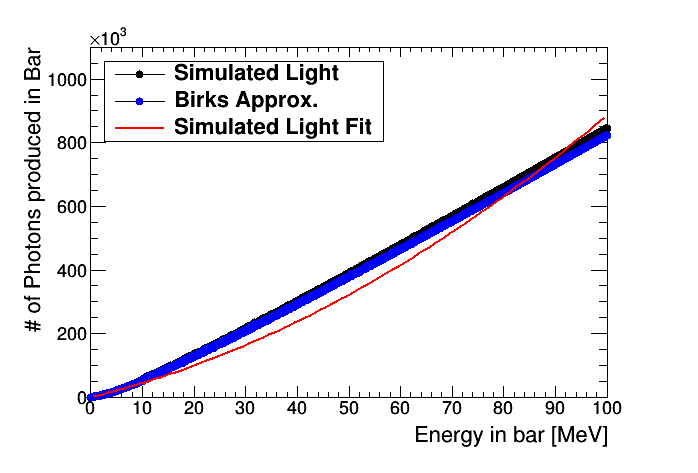
\includegraphics[width=\linewidth]{light_of_protons0-100mev.png}
  \captionsetup{width=.9\linewidth}
  \caption{proton light produced by Geant4 compared to the Birks approximation of that light, the simulated light fit is the square funciton $L = aE^2 + bE+ c$ and is fit to the Geant4 simulated light}
  \label{subFig_proton_light}
\end{subfigure}%
\begin{subfigure}{.5\textwidth}
  \centering
  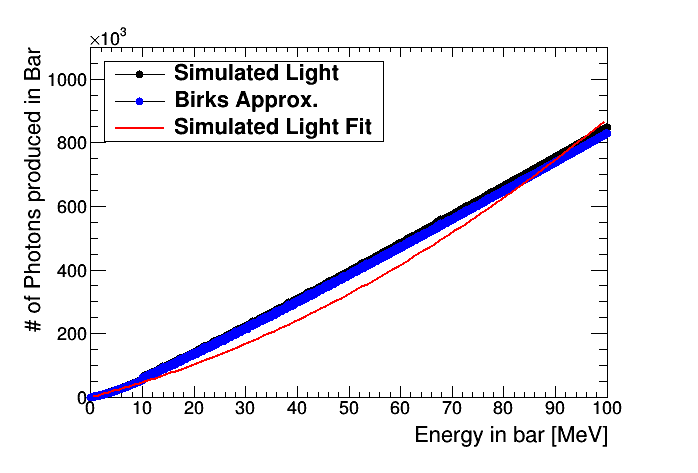
\includegraphics[width=\linewidth]{light_of_Aprotons0-100mev.png}
  \captionsetup{width=.9\linewidth}
  \caption{anti-proton light produced by Geant4 compared to the Birks approximation of that light, the simulated light fit is the square funciton $L = aE^2 + bE+ c$ and is fit to the Geant4 simulated light}
  \label{subFig_aproton_light}
\end{subfigure}
\caption{proton and anti-proton light output compared to the birks approximation and a square fit to the light out put in Geant4}
\label{fig_proton_aproton_light}
\end{figure}
However the light yield for electrons and positrons seen in figure \ref{fig_electron_positron_light} varies more significantly. A variation of $\sim$ 15\,\% is seen in the electrons, figure \ref{subFig_electron_light}, and a variation and a variation of $\sim$ 20\,\% is seen in positrons, figure \ref{sub_Figpositron_light} at maximum energy values. In figure \ref{fig_electron_positron_light}, the simulated light fit, which is a square fit to the data in the form $L = aE^2 + bE+ c$ fits the data far closer. Figure \ref{fig_square_electron_positron_light} shows this approximation inputted instead, there is a slight variation between the simulated light fit and the square approx. seen in figures \ref{subFig_square_electron_light} and \ref{subFig_square_positron_light}. This is because the simulated light fit is fitted to the whole light distribution whereas the light of the square approximation is produced per Geant4 step. Despite this, the square approximation of light for electrons ($L = 0.9347E^2 + 10340E - 0.1000$) had a variation of 0.7\,\% at maximum energy and the square approximation of the light for the positrons ($L = 0.9716E^2 + 10350E -0.1000$) had a variation of 0.3\,\% at maximum energy. 
\begin{figure}[H]
\centering
\begin{subfigure}{.5\textwidth}
  \centering
  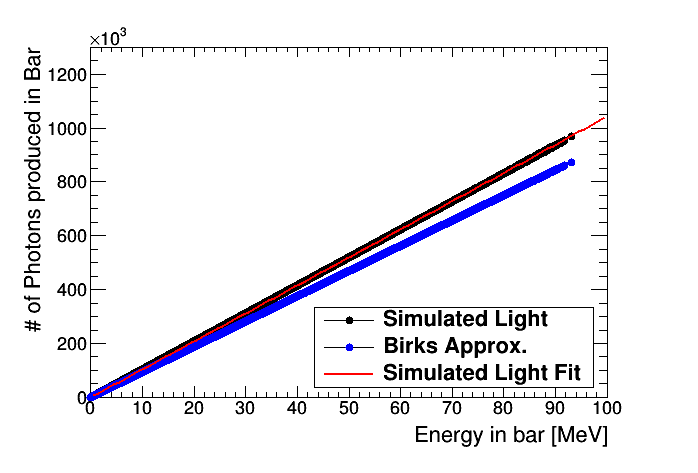
\includegraphics[width=\linewidth]{light_of_electrons0-100mev.png}
  \captionsetup{width=.9\linewidth}
  \caption{Electron light produced by Geant4 compared to the Birks approximation of that light, the simulated light fit is the square funciton $L = aE^2 + bE+ c$ and is fit to the Geant4 simulated light}
  \label{subFig_electron_light}
\end{subfigure}%
\begin{subfigure}{.5\textwidth}
  \centering
  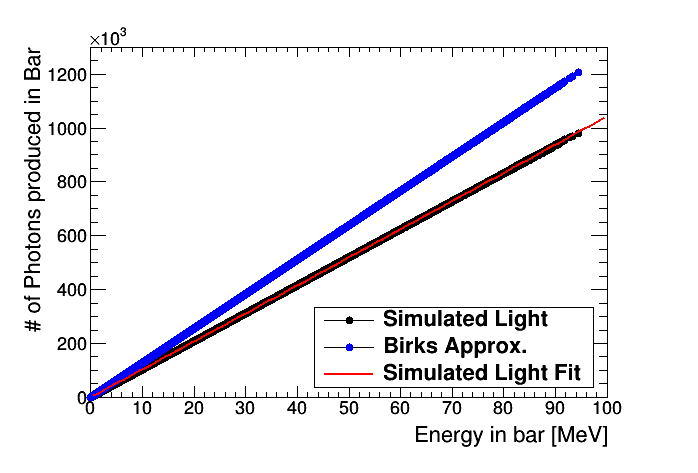
\includegraphics[width=\linewidth]{light_of_positrons0-100mev.png}
  \captionsetup{width=.9\linewidth}
  \caption{Positron light produced by Geant4 compared to the Birks approximation of that light, the simulated light fit is the square funciton $L = aE^2 + bE+ c$ and is fit to the Geant4 simulated light}
  \label{subFig_positron_light}
\end{subfigure}
\caption{Electron, Positron light output compared to the birks approximation and a square fit to the light out put in Geant4}
\label{fig_electron_positron_light}
\end{figure}
\begin{figure}[H]
\centering
\begin{subfigure}{.5\textwidth}
  \centering
  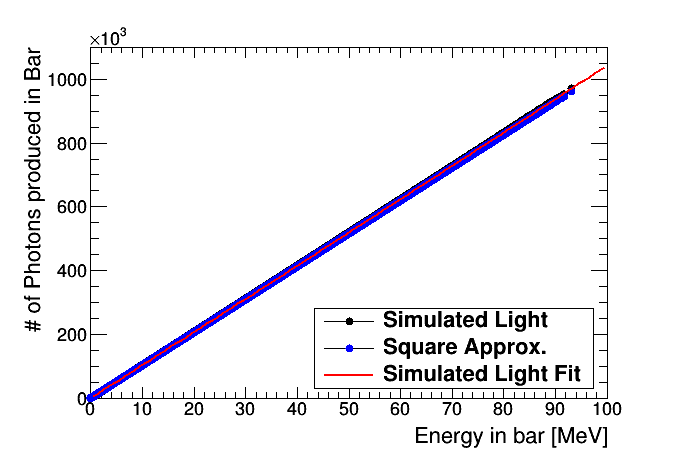
\includegraphics[width=\linewidth]{light_of_electronsLin0-100mev.png}
  \captionsetup{width=.9\linewidth}
  \caption{Electron light simulated by Geant4 compared to the square approximation $L = aE^2 + bE+ c$ }
  \label{subFig_square_electron_light}
\end{subfigure}%
\begin{subfigure}{.5\textwidth}
  \centering
  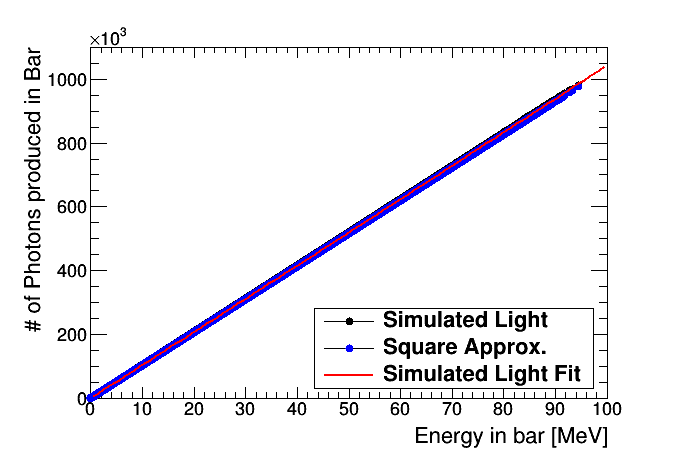
\includegraphics[width=\linewidth]{light_of_positronsLin0-100mev.png}
  \captionsetup{width=.9\linewidth}
  \caption{Positron light simulated by Geant4 compared to the square approximation $L = aE^2 + bE+ c$}
  \label{subFig_square_positron_light}
\end{subfigure}
\caption{Electron and positron light output from simulation compared to a Geant4 step square approximation}
\label{fig_square_electron_positron_light}
\end{figure}
The conversion for light into energy for electrons in figure \ref{subfig_square_electron_light} is defined by equation \ref{equ_MeV_electron_equivalent_square}. The light of an electron is the highest amount of light per MeV that a particle can deposit this MeV electron equivalent (MeVee) is a special nomenclature used to describe the absolute light yeild \cite{knoll_2010}. As the squared term $ << $ the linear term, the squared term is ignored for the purposes of light conversion, producing equation \ref{equ_MeV_electron_equivalent_linear}. By rearranging equation \ref{equ_MeV_electron_equivalent_linear} for energy production we then get equation \ref{equ_MeV_electron_equivalent_light} which allows for the conversion from the Birks approximation of light into the energy or the square approximation of light into energy for the electrons and positrons. With equation \ref{equ_MeV_electron_equivalent_light} it is possible to show the energy loss due to quenching, once the L in equation \ref{equ_MeV_electron_equivalent_light} is substituted with the light at the end of the Geant4 step shown in equation \ref{equ_light_produced}. \hl{IMPORTANT NOTE TO SELF: Again chisqs for this are very very poor, but I don't know how to make better, must return to this at a later date!} 
\begin{equation}
L = 0.9347E^2 + 10340E - 0.1000
\label{equ_MeV_electron_equivalent_square}
\end{equation}
\begin{equation}
L = 10340E - 0.1000
\label{equ_MeV_electron_equivalent_linear}
\end{equation}
\begin{equation}
E = \frac{L +0.1000}{10340} 
\label{equ_MeV_electron_equivalent_light}
\end{equation}
\subsection{Simulated Results With Physical and Electronic Effects}\label{subSec_geant4Simulation_results_physical_electronics}
\section{Cosmic Tomography}\label{sec_cosmicTomography}
\subsection{Simulation}\label{subSec_cosmicTomography_simulation}
\subsection{Methodology}\label{subSec_cosmicTomography_methodology}

%\bibliography{refs} 
%\bibliographystyle{ieeetr}
\printbibliography


\end{document}
